\section{Лекция 19}
\begin{example} [Сапог Шварца]\footnote{Взято из семинаров О.Н. Косухина на teach-in} $\\$
    Рассмотрим сечения цилиндра, проходящие на равном расстоянии друг от друга параллельно основаниям цилиндра (и два сечения будут совпадать с основаниями). Пусть между сечениями образовалось $m$ цилиндрических слоёв. В каждом сечении построим правильный $n$-угольник, вписанный в образовавшуюся окружность. Причём пусть вершины в каждом сечении (кроме самого верхнего) находятся ровно на середине дуги между соседними вершинами в соседнем сечении сверху. Соединим отрезками эти точки (а в самом нижнем сечении соединим отрезками все соседние вершины). Получим поверхность, называемую сапогом Шварца.
    \begin{center}
    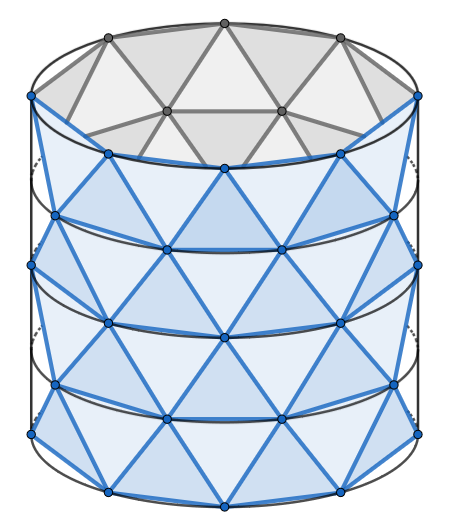
\includegraphics[width=0.3\textwidth]{Images/Sapog.png}
    \hspace{2cm}
    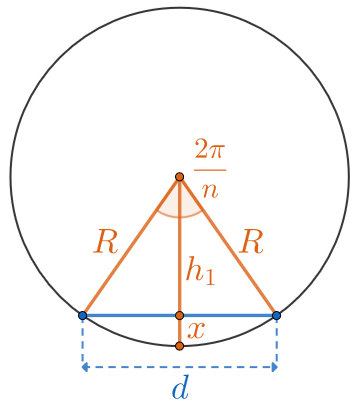
\includegraphics[width=0.3\textwidth]{Images/Sapogwork.png}
    \end{center}
    В каждом слое сапога Шварца находится $2n$ треугольников, тогда вся эта поверхность состоит из $2nm$ треугольников. Обозначим $d$ основания треугольников, являющиеся хордами окружностей.
    \[d=2R\cdot \sin{\frac{\pi}{n}},\ \ h_1=R\cdot \cos\frac{\pi}{n},\ \ x=R\left(1-\cos{\frac{\pi}{n}}\right)\]
    Тогда по теореме Пифагора можем найти высоту $h_2$ треугольника из поверхности сапога Шварца:
    \[h_2=\sqrt{\left(\frac{h}{m}\right)^2+R^2\left(1-\cos{\frac{\pi}{n}}\right)}\]
    Где $h$ --- высота цилиндра. Значит площадь поверхности сапога Шварца равна:
    \begin{multline*}
        S=2mn\cdot \frac{1}{2}\cdot 2R\cdot\sin{\frac{\pi}{n}}\cdot \sqrt{\left(\frac{h}{m}\right)^2+R^2\left(1-\cos{\frac{\pi}{n}}\right)}=\\
        =2\pi R\cdot \cfrac{\sin{\frac{\pi}{n}}}{\frac{\pi}{n}}\cdot \sqrt{h^2+R^2m^2\left(1-\cos{\frac{\pi}{n}}\right)^2}
    \end{multline*}
    При $m,n\to +\infty$:
    \[\cfrac{\sin{\frac{\pi}{n}}}{\frac{\pi}{n}}\to 1\]
    но $m\left(1-\cos{\frac{\pi}{n}}\right)$ может стремиться к любому наперёд заданному неотрицательному числу (или к $+\infty$) в зависимости от относительного характера стремления $m$ и $n$. Таким образом, S может стремиться к любому наперёд заданному числу, не меньше $2\pi Rh$ (или к $+\infty$).
\end{example}
\begin{theorem}[Достаточное условие потенциального поля в односвязной области]
    Пусть $F=(P,Q)$ --- векторное поле, $\Omega\subset \R^2$ --- односвязная область и\\
    $\partial \Omega$ --- связное множество. Тогда если $(P,Q)\in \mathcal{D}(\Omega)$ и $Q'_x=P'_y$, то\\
    $(P,Q)$ --- потенциальное поле.
\end{theorem}
\begin{proof}
    Пусть $\gamma$ --- произвольная замкнутая ломаная без самопересечений, лежащая в $\Omega$, обозначим $\Phi$ --- область, которую ограничивает $\gamma$. Тогда по формуле Грина:
    \[\int\limits_{\gamma}P\ dx+Q\ dy=\iint\limits_{\Phi}(Q'_x-P'_y)\ dxdy=0\]
    Значит по теореме \ref{potential} известно, что $(P,Q)$ --- потенциальное поле.
\end{proof}
\begin{example} 
    Условие односвязности области $\Omega$ нельзя опустить. Пусть\\
    $\Omega=\{(x,y): 0<x^2+y^2<R\}$. Возьмем 
    \[P=\frac{y}{x^2+y^2},\ \ Q=\frac{-x}{x^2+y^2}\]
    \[P'_y=\frac{x^2-y^2}{(x^2+y^2)^2},\ \ Q'_x=\frac{x^2-y^2}{(x^2+y^2)^2}\ \Rightarrow\ P'_y=Q'_x\]
    \[\oint\limits \frac{x\ dy-y\ dx}{x^2+y^2}=\Bigg|
        \begin{matrix}
            x=r\cdot \cos{\phi}\\
            y=r\cdot \sin{\phi}
        \end{matrix}\Bigg|=\frac{1}{r^2}\cdot \int\limits_{0}^{2\pi}r^2\cdot \cos^2{\phi}+r^2\cdot \sin^2{\phi}\ d\phi=2\pi\neq 0\]
\end{example}
\subsection{Поверхности в $\R^n$}
\textit{тут что то про поверхности}
\begin{definition}\tab
    \begin{enumerate}
        \item Пусть $\Omega\subset\R^2,\ \partial\Omega=\gamma$ --- кусочно-гладкая кривая. Отображение
        $\phi:\overline{\Omega}\to\R^k$, где $k\geq 3$ такое, что $\phi\in \mathcal{C}^1(\overline{\Omega})$
        \[\phi(u,v)=(x_1(u,v),\dots,x_k(u,v))\]
        и в $\Omega$:
        \[\text{rk}\begin{pmatrix}
            \phi'_u\\
            \phi'_v
        \end{pmatrix}=2\]
        называется гладкой параметризацией поверхности.
        \item Пусть $\phi_1: \Omega_1\to \R^k,\ \phi_2: \Omega_2\to \R^k$. Считаем, что $\phi_1$ и $\Phi_2$ эквивалентны (параметризуют одну и ту же поверхность), есть существует биективная $\psi:\Omega_1\to \Omega_2$ такая, что $\det{J_{\psi}}\neq 0$ на $\Omega_1$ и $\phi_2\equiv\phi_1\circ\psi$.
        \item Поверхностью называется класс эквивалентности гладких параметризаций по указанному отношению.
    \end{enumerate}
\end{definition}
\begin{comm}
    Пусть
    \[r(u,v)=(x_1(u,v),\dots,x_k(u,v))\in \mathcal{C}^1(\overline{\Omega})\]
    введем
    \[r'_u=((x_1)'_u,\dots,(x_k)'_u),\ r'_v=((x_1)'_v,\dots,(x_k)'_v)\]
    и потребуем, чтобы эти векторы были линейно независимыми, то есть
    \[\text{rk}\begin{pmatrix}
        (x_1)'_u & \dots & (x_k)'_u\\
        (x_1)'_v & \dots & (x_k)'_v
    \end{pmatrix}=2\]
    В параметризации $r(u,v)$ в каждой точке поверхности определен дифференциал --- линейное отображение $dr:\R^2\to\R^k$ такое, что 
    \[dr(du,dv)=r'_u\ du+r'v\ dv\] 
    Рассмотрим прямоугольник со сторонами $\Delta u$ и $\Delta v$. Образом этого прямоугольника при линейном отображении $dr$ будет параллелограмм, натянутый на векторы 
    \[a=dr(\Delta u,0)=r'_u \Delta u,\ \ b=dr(0,\Delta v)=r'_v \Delta v\]
    Найдем его площадь
    \begin{multline*}
        S_{\{a,b\}}=\|a\|\cdot \|b\|\cdot \sin{\alpha}=\|r'_u\|\cdot \Delta u\cdot \|r'_v\|\cdot \Delta v\cdot \sqrt{1-\cos^2{\alpha}}=\\
        =\|r'_u\|\cdot \Delta u\cdot \|r'_v\|\cdot \Delta v\cdot \sqrt{1-\left(\frac{r'_u\cdot r'_v}{\|r'_u\|\cdot \|r'_v\|}\right)^2}=\\
        =\sqrt{\|r'_u\|^2\cdot \|r'_v\|^2-(r'_u\cdot r'_v)^2}\ \Delta u\Delta v=\sqrt{EG-F^2}\ \Delta u\Delta v
    \end{multline*}
    где ввели обозначения
    \[E=\|r'_u\|^2=r'_u\cdot r'_u,\ F=r'_u\cdot r'_v,\ G=\|r'_v\|^2=r'_v\cdot r'_v\]
\end{comm}
\begin{definition}
    Площадью гладкой поверхности $\Sigma$ назовем 
    \[|\Sigma|=\iint\limits_{\overline{\Omega}}\sqrt{EG-F^2}\ dudv\]
\end{definition}
\begin{theorem}
    Площадь поверхности не зависит от параметризации.
\end{theorem}
\begin{proof}
    Без доказательства.
\end{proof}
\subsection{Поверхностный интеграл первого рода}
\begin{definition}
    Пусть $\Omega$ область в $\R^2$, $\phi:\Omega\to\R^k$ --- параметризация поверхности $\Sigma$ и функция $f(x,y,z)$ определена на $\phi(\overline{\Omega})$. Тогда интеграл
    \[\iint\limits_{\Sigma}f(x,y,z)dS:=\iint\limits_{\overline{\Omega}}f(x(u,v),y(u,v),z(u,v))\cdot \sqrt{EG-F^2}\ dudv\]
    называется поверхностным интегралом первого рода.
\end{definition}
\begin{comm}
    Пусть поверхность $\Sigma$ задается графиком функции:
    \[\begin{cases}
        x=u\\
        y=v\\
        z=z(x,y)
    \end{cases}\]
    Для этого случая:
    \[r'_x=(1,0,z'_x),\ \ r'_y=(0,1,z'_y)\]
    \[E=1+(z'_x)^2,\ F=z'_x\cdot z'_y,\ G=1+(z'_y)^2\]
    \[EG-F^2=(1+(z'_x)^2)(1+(z'_y)^2)-(z'_x\cdot z'_y)^2=1+(z'_x)^2+(z'_y)^2\]
    Значит, если поверхность $\Sigma$ задается графиком функции, то 
    \[\iint\limits_{\Sigma}f\ dS=\iint\limits_{\overline{\Omega}}f(x,y,z(x,y))\cdot \sqrt{1+(z'_x)^2+(z'_y)^2}\ dxdy\]
    % Напишем уравнение касательной плоскости в точке $(x_0,y_0,z_0)$:
    % \[z-z_0=z'_x(x_0,y_0)(x-x_0)+z'_y(x_0,y_0)(y-y_0)\]
\end{comm}
\noindent Приведем несколько свойств, следующих из определения:
\begin{statement}
    Если $f\in \mathcal{C}(\phi(\overline{\Omega}))$, то существует интеграл
    \[\iint\limits_{\Sigma}f\ dS\]
\end{statement}
\begin{statement}
    Пусть существуют интегралы
    \[\iint\limits_{\Sigma}f\ dS,\ \iint\limits_{\Sigma}g\ dS\]
    Тогда $\forall c_1,c_2\in \R$ существует интеграл
    \[\iint\limits_{\Sigma}(c_1\cdot f+c_2\cdot g)\ dS=c_1\cdot \iint\limits_{\Sigma}f\ dS+c_2\cdot \iint\limits_{\Sigma}g\ dS\]
\end{statement}
\begin{statement}
    Поверхностный интерал первого рода не зависит от ориентации.
\end{statement}
\begin{statement}
    Пусть $f(\overline{x})\leq g(\overline{x})$ для всех $\overline{x}\in \phi(\overline{\Omega})$. Тогда 
    \[\iint\limits_{\Sigma}f\ dS\leq \iint\limits_{\Sigma}g\ dS\]
\end{statement}
\begin{statement}
    \[\left|\iint\limits_{\Sigma}f\ dS\right|\leq \sup|f|\cdot |\Sigma|\]
\end{statement}
\begin{proof}
    \begin{multline*}
        \left|\ \iint\limits_{\Sigma}f\ dS\ \right|\leq \iint\limits_{\Omega}|f(x(u,v),y(u,v),z(u,v))|\cdot\sqrt{EG-F^2} \leq\\
        \leq \sup|f|\cdot \iint\limits_{\Omega}\sqrt{EG-F^2} = \sup|f|\cdot |\Sigma|
    \end{multline*}
\end{proof}
\newpage